\documentclass{article}
    \usepackage[utf8]{inputenc} %caratteri speciali tastiera come "ç"
    \usepackage{enumerate}
    \usepackage{lmodern}
    \usepackage{calligra}
    \usepackage{accanthis}
    \usepackage[T1]{fontenc} %codifica font
    \usepackage[italian]{babel} %lingua del documento
    \usepackage{graphicx}
    \usepackage{listings}
    \usepackage{geometry}
    \geometry{a4paper, left=2cm, right=2cm, top=2.5cm, bottom=2cm}
    \usepackage{titlesec}
    \titleformat{\section}
    [hang]
    {\usefont{T1}{lmodern}{}{}\bfseries\centering\Large\itshape}
    {\thesection.}{0.5em}{\vspace{0.5ex}}[\vspace{0.5ex}]

\begin{document}
\begin{titlepage}
    \centering
    
\includegraphics[scale=0.2]{img/swe.jpg}
    \par\vspace{3cm}
    { \fontsize{60}{1}\selectfont Glossario SWE}
    \par\vspace{5cm}
    {\usefont{T1}{calligra}{}{} \fontsize{40}{1}\selectfont Mihai Eni }
    \vfill
    {\Large{2018/2019}}
\end{titlepage}

\tableofcontents
\newpage

\section{Primo capitolo}

    \subsection{Metodo di lavoro necessario per la professione informatica:}
        Il metodo di lavoro di un informatico si divide nelle seguenti 4 fasi:ù
        \begin{enumerate}[I]
            \item \textit{Gestire il tempo}: richiede la capita di organizzare il proprio tempo per rispettare le disponibilità e le scadenze, ioltre si chiede di poter organizzarsi in base alle proprieta e ai conflitti;
            \item \textit{Collaborare}: vengono fissati degli obiettivi, si dividono i compiti tra i vari componenti e richiede di verficare i progressi ottenuti da ciascun componente; 
            \item \textit{Assumersi responsabilità}: richiede di rispettare le scadenze e riportare le difficoltà incontrate;
            \item \textit{Auto-aprendimento}: "imparare a imparare" cioè la capita di apprendere in modo autonomo nuovo conoscenze come: l'utilizzo di una nuova tecnologià mai vista prima.
            \end{enumerate}
    \subsection{Glossario}
        Raccolta di termini e concetti che hanno la necessita di spiegazione, dove viene fornita la specifica del loro signaficato e ogni altra informazione utile alla comprensione del loro significato,inoltre vengono registrati in un ordine che ne faciliti la localizzazione.
    \subsection{Progetto}
        È un insieme di attività e compiti \footnote{attività $\ne$ compiti in quanto i compiti sono una parte primitiva delle attività} con le seguenti proprieta:
        \begin{itemize}
            \item raggiungere determinati obiettivi con specifiche fissate;
            \item hanno una durata fissata la quale deve essere rispetata;
            \item hanno a disposizione una quatita limitata di riorse (\textit{persone, tempo, soldi, strumenti, ect});
            \item utilizzano le risorse durante il loro svolgimento.  
            \end{itemize}
        Contenente le seguenti principali attività:
        \begin{enumerate}[I]
            \item \textbf{Pianificazione}: gestire le risorse e le responsabilità;
            \item \textbf{Analisi dei requisiti}: definire cosa bisogna fare;
            \item \textbf{Progettazione}: definire come farlo;
            \item \textbf{Realizzazione}:
            \begin{itemize}
                \item fare quello che serve mirando alla qualità; 
                \item controllare quello che si produce affinche non contenga errori;
                \item verficare la validità dei risultati rispetto alle attese.
                \end{itemize}
            \end{enumerate}
        \begin{figure}[!h]      
            \centering  
            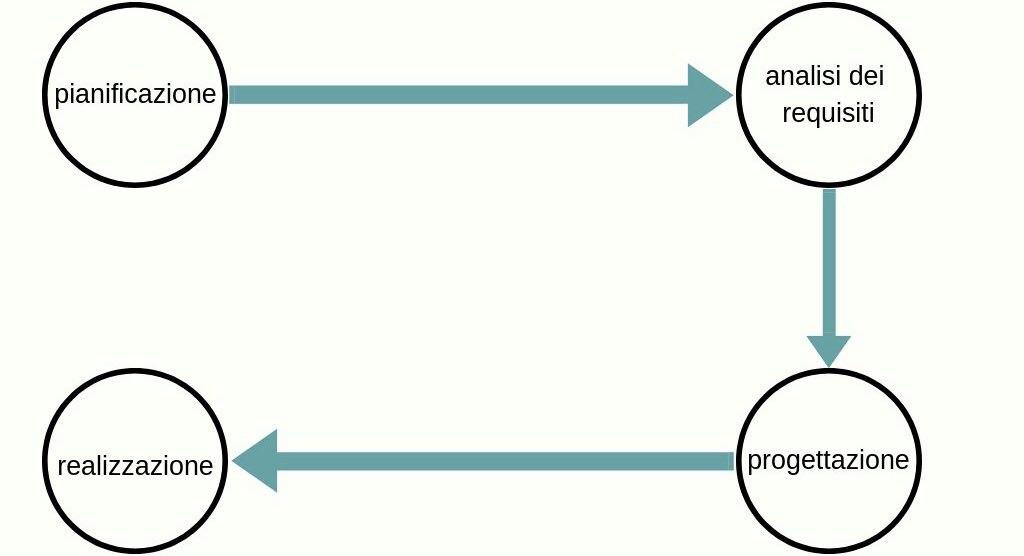
\includegraphics[height=14em,width=15cm]{img/attivita.jpg}
            \end{figure}
            

\end{document}
